\chapter{\introductionname}
\newpage
\begin{parskipenv}
Hoy en día, las auditorías de seguridad forman parte esencial de la estrategia de ciberseguridad de cualquier organización. Su finalidad es identificar, evaluar y mitigar vulnerabilidades que puedan ser explotadas por agentes maliciosos. Para lograrlo, estas auditorías se estructuran en distintas fases que emulan el comportamiento de un atacante real, lo que permite analizar el estado de seguridad de los sistemas desde una perspectiva ofensiva.

Una auditoría de seguridad suele desarrollarse de forma secuencial, siguiendo un conjunto de etapas reconocidas en las metodologías profesionales más adoptadas en el sector. Estas fases \cite{fases_auditoria} son las siguientes:

\begin{enumerate}
  \item \textbf{Reconocimiento}: Recopilación pasiva o activa de información sobre el objetivo (direcciones IP, dominios, tecnologías empleadas, subdominios, etc.), que servirá para planificar los ataques posteriores.
  
  \item \textbf{Escaneo}: Identificación de servicios activos, versiones, puertos abiertos y posibles vulnerabilidades que puedan ser explotadas.
  
  \item \textbf{Obtención de acceso}: Explotación de las vulnerabilidades detectadas en la fase anterior para obtener acceso al sistema, ya sea mediante credenciales débiles, fallos de configuración o ejecución de exploits.
  
  \item \textbf{Mantenimiento del acceso}: Aplicación de técnicas para mantener el control del sistema comprometido, como la instalación de puertas traseras (backdoors) o la creación de cuentas persistentes.
  
  \item \textbf{Borrado de huellas}: Eliminación de registros, logs y cualquier otra evidencia que pueda alertar a los administradores del sistema de la intrusión realizada.
  
  \item \textbf{Informe}: Elaboración de un documento técnico que recoja todo el proceso llevado a cabo, incluyendo las vulnerabilidades encontradas, su criticidad, las evidencias obtenidas y las recomendaciones para corregir los problemas detectados.
\end{enumerate}

Como se puede observar, la fase de \textbf{reconocimiento} representa el punto de partida de todo el proceso. A partir de la información recolectada en esta etapa, el auditor podrá construir una visión detallada del entorno y prepararse para fases posteriores como el escaneo o la explotación. Por ello, optimizar esta fase resulta fundamental para garantizar la eficacia y la calidad de toda la auditoría.

Esta fase es una de las más importantes dentro de una auditoría. Tiene como objetivo recopilar la máxima cantidad de información posible sobre el objetivo a analizar \cite{recon}. A partir de estos datos, el auditor puede identificar servicios expuestos, tecnologías empleadas y potenciales vectores de ataque, sentando así las bases para etapas más avanzadas como la explotación.

A pesar de su importancia, las tareas asociadas al reconocimiento suelen ser repetitivas, tediosas y propensas a errores si se realizan manualmente. Además, muchas de las herramientas empleadas requieren conocimientos técnicos, uso de línea de comandos y un esfuerzo considerable para gestionar los resultados obtenidos. Este escenario genera una necesidad clara de soluciones que permitan automatizar este proceso, reducir los tiempos de ejecución y facilitar la gestión de la información recopilada.

El presente Trabajo de Fin de Grado surge como respuesta a esta problemática. Se ha desarrollado una herramienta que automatiza las tareas fundamentales de reconocimiento en una auditoría de seguridad, integrando distintas utilidades en un único entorno con interfaz gráfica. Esta solución permite realizar desde escaneos de puertos y servicios hasta la enumeración de subdominios, identificación de vulnerabilidades web, detección de CMS y análisis de servicios como FTP o SSH. Además, la herramienta permite interactuar con un sistema de inteligencia artificial basado en modelos generativos, que facilita la interpretación de resultados y la propuesta de acciones posteriores.

Entre las funcionalidades añadidas destacan también la generación automática y versionada de informes, la configuración de escaneos exhaustivos, la personalización del entorno mediante proxies y un sistema de proyectos que organiza los análisis por objetivo.

La herramienta está diseñada con una arquitectura modular y escalable, lo que permite incorporar en un futuro nuevas funcionalidades de forma sencilla. Esto la convierte en una solución con capacidad para seguir evolucionando y ampliándose mediante la integración de nuevos módulos que permitan cubrir un mayor número de servicios y casos de uso.

Durante el desarrollo se han evaluado múltiples alternativas tecnológicas, priorizando aquellas que ofrecieran un equilibrio entre rendimiento, actualización activa, facilidad de integración y compatibilidad. Herramientas como Nmap, Subfinder, Nuclei, WPScan o Feroxbuster han sido seleccionadas tras un análisis comparativo, mientras que otras como Nikto, Gobuster o Paramiko fueron descartadas por distintos motivos técnicos.

El resultado es una herramienta funcional, útil y extensible, capaz de reducir significativamente el tiempo y la carga de trabajo durante la fase de reconocimiento, agilizando así el proceso de auditoría y mejorando la calidad del análisis desde las primeras etapas.

La figura \ref{fig:fases_auditoria} ilustra las distintas fases de una auditoría de seguridad ofensiva, destacando la importancia del reconocimiento como punto de partida y fase en la que se centra esta herramienta.

\begin{figure}[H]
\centering
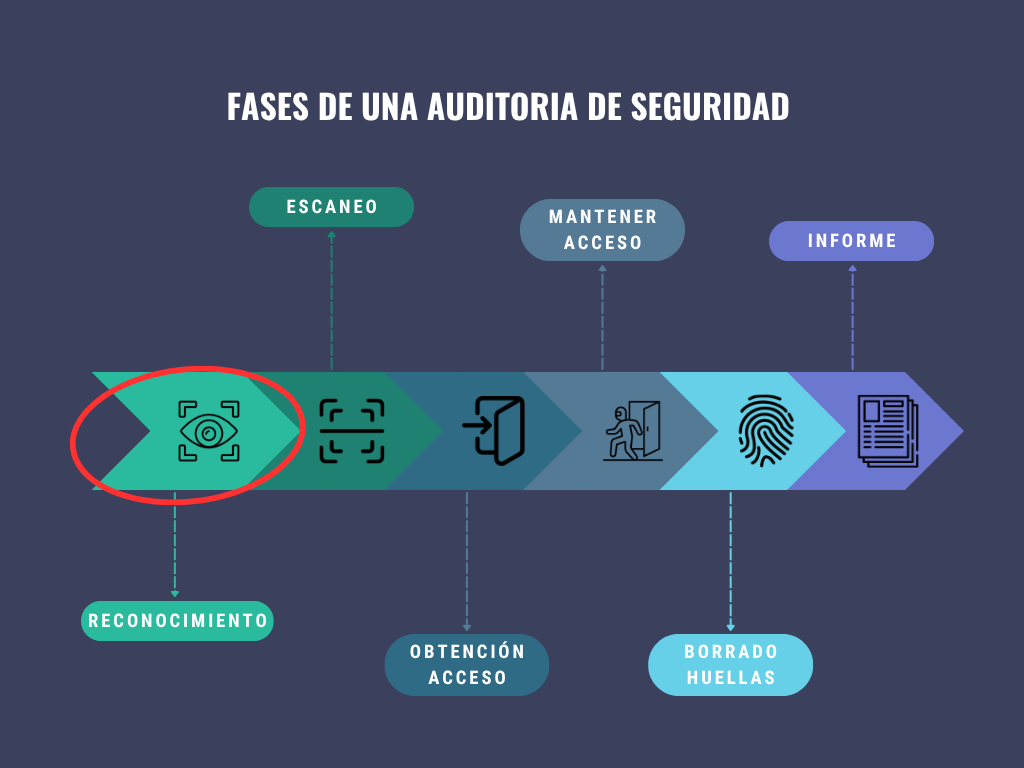
\includegraphics[width=\textwidth]{pictures/fasesAuditoria.png}
\caption{Fases de una auditoría de seguridad ofensiva.}
\label{fig:fases_auditoria}
\end{figure}

\section{Estructura del documento}
Este documento se encuentra estructurado en siete capítulos, además de las correspondientes referencias bibliográficas. A continuación, se describe brevemente el contenido de cada uno de ellos:

\begin{itemize}
    \item El \textbf{Capítulo 2} recoge los objetivos que se pretenden alcanzar con el desarrollo de la herramienta propuesta.
    
    \item El \textbf{Capítulo 3} presenta el estado del arte, en el que se analizan las principales herramientas existentes en el ámbito del reconocimiento automatizado y se identifican sus principales limitaciones.
    
    \item El \textbf{Capítulo 4} describe la metodología seguida para el desarrollo de la herramienta, justificando la elección de cada tecnología empleada y explicando el flujo de trabajo que se implementa durante el proceso de reconocimiento.
    
    \item El \textbf{Capítulo 5} detalla el proceso de implementación de la herramienta, desde el diseño de su arquitectura hasta la integración de sus distintos módulos.
    
    \item El \textbf{Capítulo 6} recoge los resultados obtenidos a partir de las pruebas realizadas sobre distintos escenarios, evaluando la eficacia de la herramienta y el cumplimiento de los objetivos definidos.
    
    \item El \textbf{Capítulo 7} expone las conclusiones extraídas del trabajo, así como posibles líneas futuras de mejora y ampliación del sistema desarrollado.
    
    \item Finalmente, se incluyen las \textbf{referencias bibliográficas} consultadas a lo largo del proyecto. % Y posible Anexo??
\end{itemize}

\end{parskipenv}